% !TeX spellcheck = en_GB
\section{Modular Forms Modulo Two}
\subsection{Strategy to Reduce Modulo Two}
It is not trivial, at this point, why and how we can reduce modulo 2 modular forms, objects that have coefficients in $\C$.
In general, reduction modulo a number is only possible with whole numbers (integers).
We would like to reduce modulo 2 coefficients of the Fourier series for modular forms.
But at the moment, they lie in $\C$.

In fact, we will introduce a new basis for the modular forms: the so called Miller Basis.
The coefficients of all the forms in this basis are integers. It is then possible to consider the space of modular forms over $\Z$ instead of $\C$.
Once this is done, we will reduce all the newly integral coefficients modulo $2$.

In this section, we will denote all objects reduced modulo 2 with an $\overline{\text{over-line}}$:
\begin{itemize}
	\item The modular form $f$ once reduced will be denoted $\overline{f}$.	\item The coefficients of the $q$-expansion $c$ will reduce to $\overline{c}$
	\item The Hecke operators $T_n$ reduced will be denoted $\overline{T_n}$.
\end{itemize}

\subsection{Integral Basis}
\subsubsection{Normalisation of Typical Modular Forms}
\paragraph{Normalisation of Eisenstein series $G_k$}
We first recall the formula for $q$ extension of $G_k$ and the one for $\zeta(2k)$:
$$
G_k(q) = 2\zeta(2k) + 2 \frac{{(2 \pi i)}^{2k}}{(2k-1)!} \sum_{n=1}^{\infty} \sigma_{2k-1}(n)q^n
$$
and
$$
2\zeta(2k) = \frac{(2\pi)^{2k}}{(2k)!}B_k,
$$
so overall:
$$
G_k(q) = \frac{(2\pi)^{2k}}{(2k)!}B_k + 2 \frac{{(2 \pi i)}^{2k}}{(2k-1)!} \sum_{n=1}^{\infty} \sigma_{2k-1}(n)q^n.
$$

We would like to normalize this series, so that the coefficients become integers, so that we can ultimately reduce them modulo 2.
Right now, coefficients are rational.

As we want to keep the series modular with same weight, the only tool we have to normalize the series is multiplication by a constant.
The normalization is a crucial point: if we multiply by $2$ all coefficients of a modular form that already lie in $\Z$, the reduction modulo 2 will always give zero.

First, let's normalize the series to have particular values on some coefficients of interest.
There are two justified ways to do so: normalize to have constant ($q^0$) coefficient set to one, and to have $q^1$ coefficient set to one.
We will introduce both:
We define $E_k$ be such that:
$$
E_k \cdot 2\zeta(2k) = G_k,
$$
so that
$$
E_k = 1 + (-1)^k \frac{4k}{B_k} \sum_{n=1}^{\infty} \sigma_{2k-1}(n)q^n.
$$
$E_k$ then has constant coefficient set to 1.

We also define $F_k$ be such that:
$$
F_k \cdot \left( 2 \frac{{(2 \pi i)}^{2k}}{(2k-1)!} \right) = G_k,
$$
so that
$$
F_k =  (-1)^k \frac{B_k}{4k} + \sum_{n=1}^{\infty} \sigma_{2k-1}(n)q^n.
$$
$F_k$ then has $q$-coefficient set to 1 (as $\sigma_{2k-1}(1)=1$).

Clearly, the coefficients of this expansion remain in $\Q$ at least, and we will show that for some specific $k$, the coefficients lie in fact in $\Z$.
Both $F_k$ and $E_k$ are interesting, but for our purpose (reducing modulo 2), we will use $E_k$.
Note that $E_k$ are normalized versions of Eisenstein series $G_k$, but in literature, both are called Eisenstein series; see \cite[p.6]{IntoductionModularFormsWorkshop} for example.

\paragraph{The Modular Discriminant $\Delta$ Normalized}
Again, we recall the formula for $q$ extension of $\Delta$:
$$
\Delta(q) = q \prod_{n=1}^{\infty} (1-q^n)^{24}.
$$
Clearly, the coefficients in expansion of $\Delta$ are integers (which we can reduce modulo 2).
This is the reason why we defined $\Delta$ with the $\frac{1}{(2\pi)^{12}}$ factor in front.


\subsubsection{Miller Basis}
\paragraph{Basis with Integral Coefficients (in Fourier Series)}
Applying normalization $G_k \mapsto E_k$ above for $k=2,3$, we get:
\begin{align*}
	E_2 &= 1 + \frac{8}{B_2} \sum_{n=1}^{\infty} \sigma_{3}(n)q^n \qquad B_2 = \frac{1}{30} \\
	    &= 1 + 240 \sum_{n=1}^{\infty} \sigma_{3}(n)q^n
\end{align*}

and
\begin{align*}
	E_3 &= 1 - \frac{12}{B_3} \sum_{n=1}^{\infty} \sigma_{5}(n)q^n \qquad B_3 = \frac{1}{42} \\
	    &= 1 - 504 \sum_{n=1}^{\infty} \sigma_{5}(n)q^n
\end{align*}

Now, we have shown that $\{G_2^aG_3^b \mid 2a+3b=k\}$ is a basis for modular forms of weight $2k$ over the complex (see \ref{BasisModularForms}).
As $E_2 = \lambda G_2,\ \lambda \in \C$ and $E_3 = \mu G_3,\ \mu \in \C$, we have that $\{E_2^aE_3^b \mid 2a+3b=k\}$ remains a basis for $M_k$ over $\C$.

It is clear, from the series, that coefficients of the $q$-expansion of both $E_2$ and $E_3$ are all integers.
Thus, so are coefficients of combinations of $E_2$ and $E_3$.
Therefore, we have found a basis for $M_k$ such that all elements in the basis have only integral coefficients in their $q$-expansion.
\label{IntegralBasisModularForms}

\paragraph{Miller Basis for $M_k^0$}
This is a nice result, but we can in fact do better, by forcing the first coefficients to chosen values.

\begin{theorem}
	For the space of modular cusp forms $M_k^0$, there exists a basis $\{f_1, \cdots, f_r\}$ such that:
	\begin{itemize}
		\item $f_i \in \Z[[q]]$
		\item $ a_i^j = \delta_{ij} = 
		\left\lbrace
		\begin{array}{l l}
			1 & \text{ if } i   =  j \\
			0 & \text{ if } i \neq j
		\end{array}
		\right. \quad
		\forall 1 \leq i,j \leq r$\\
		where $a_i^j$ is the coefficient of $q^j$ in expansion of $f_i$.
	\end{itemize}
\end{theorem}
This is commonly called the Miller basis for $M_k^0$, as it was first introduced by Victor Saul Miller \cite{MillerThesis}.
\begin{proof}
	\begin{itemize}
		%boring part
		\item For $k<6$, $k=7$, we have $\dim(M_k^0)=0$.
		Thus, $\emptyset$ is a basis which satisfies the Miller basis properties.
		
		%semi-boring part
		\item For $k=6$, we have $\dim(M_k^0)=1$.
		Thus, $\{ \Delta \}$ is a basis which satisfies the Miller basis properties.
		
		%interesting part
		\item For $k \geq 7$, we let $r = \dim(M_k^0) \geq 1$.	
		We then consider the set $\{ g_j \mid 1 \leq j \leq r \}$ where
		$$
		g_j = \Delta^jE_3^{2(d-j)+b}E_2^a
		$$
		with $2a+3b \leq 7$, $2a+3b \cong k \bmod 6$ and $d = \frac{k-(2a+3b)}{6} \in \N$ (with $k \geq 7$).
		Note that $a$ and $b$ are unique unless $k \cong 0 \bmod 6$. In witch case, we use by convention $a=0$, $b=0$.
		As all $E_2$, $E_3$, and $\Delta$ have integral coefficients, $g_j$ will as well.
		
		We then look at the $q$-series
		$$
		\Delta(q) = q + \mathcal{O}(k^2) \implies \Delta^j(q) = q^j + \mathcal{O}(k^{j+1}).
		$$
		As we normalized, we have
		$$
		E_2(q) = 1 + \mathcal{O}(q) \implies E_2^{\alpha}(q) = 1 + \mathcal{O}(q)
		$$
		$$
		\text{ and } E_3(q) = 1 + \mathcal{O}(q) \implies E_3^{\alpha}(q) = 1 + \mathcal{O}(q).
		$$
		
		This gives:
		$$
		g_j(q) = q^j + \mathcal{O}(q^{j+1}) \quad \forall 1 \leq j \leq r.
		$$
		Therefore, $\{ g_j \mid 1 \leq j \leq r \}$ is clearly a linearly independent set. By dimension argument, it also spans $M_k^0$. Therefore, it forms a basis.
		Moreover, in this basis: $a_i^j = \delta_{ij} \quad i \leq j$.
		
		Now, viewing $\Delta$-coefficients of the modular forms $\{g_j\}$ as rows of a matrix, we can perform Gaussian elimination on them.
		We will obtain a basis $\{f_j \mid 1 \leq j \leq r \}$ such that: $a_i^j = \delta_{ij} \text{ for all } 1 \leq i,j \leq r$.
		The coefficients will remain in $\Z$.
	\end{itemize}
\end{proof}

\paragraph{Extension to all $M_k$}
We already have a basis for $M_k^0$, as $\dim(M_k) = \dim(M_k^0) + 1$ (over $\C$), we just need to adjoint one element of $M_k \setminus M_k^0$ to our basis.
It was shown before that $\{E_2^aE_3^b \mid 2a+3b=k\}$ is a basis for $M_k$ with integral coefficients (see \ref{IntegralBasisModularForms}).
One may see from the $q$-expansion that $E_2^aE_3^b = 1 + O(q)$ so $E_2^aE_3^b \in M_k \setminus M_k^0$.
Therefore, we can just add one element of $\{E_2^aE_3^b \mid 2a+3b = k\}$ to the Miller basis, and use Gaussian elimination again.
We get a basis for $M_k$ of the form $\{f_j \mid 0 \leq j \leq r \}$ such that in this basis: $a_i^j = \delta_{ij} \text{ for all } 0 \leq i,j \leq r$ (with $r=\dim(M_k^0)$ i.e. $r+1=\dim(M_k)$).

\paragraph{Miller Basis Examples}
\subparagraph{Miller basis for $k=16$}
We can calculate the Miller basis for $k=16$:
$k \cong 4 \bmod 12$ so $a=2$ and $b=0$; $d=2$.
We put $g_1 = \Delta^1E_3^2E_2^2$, so:
\begin{align*}
    g_1(q) &= \Delta(q)E_2^2(q)E_3^2(q)\\
           &= \left[ q - 24q^2 + 252q^3 + O(q^4) \right]\\
           & \qquad \cdot \left[ 1 + 240q + 2160q^2 + 6720q^3 + O(q^4) \right]^2\\
           & \qquad \qquad \cdot \left[ 1 - 504q - 16632q^2 + 122976q^3 + O(q^4) \right]^2\\
           &= q - 552q^2 - 188244q^3 + O(q^4)
% (Wolfram|Alpha) develop (q - 24q^2 + 252q^3)(1 + 240q + 2160q^2 + 6720q^3)^2(1 - 504q - 16632q^2 + 122976q^3)^2
\end{align*}
and $g_2 = \Delta^2E_3^0E_2^2$, so:
\begin{align*}
    g_2(q) &= \Delta^2(q)E_2^2(q)\\
           &= \left[ q - 24q^2 + 252q^3 + O(q^4) \right]^2\\
           & \qquad \cdot \left[ 1 + 240q + 2160q^2 + 6720q^3 + O(q^4) \right]^2\\
           &= q^2 + 432q^3 + O(q^4)
% (Wolfram|Alpha) develop (q - 24q^2 + 252q^3)^2(1 + 240q + 2160q^2 + 6720q^3)^2
\end{align*}
Then, $f_2=g_2$ and $f_1=g_1+552g_2$, so:
\begin{align*}
    f_1(q) &= q - 552q^2 - 188244q^3 + O(q^4) \ + \ 552 \cdot \left[q^2 + 432q^3 + O(q^4)\right] \\
           &= q + 50220q^3 + O(q^4)\\
    f_2(q) &= q^2 + 432q^3 + O(q^4)\\
% (Wolfram|Alpha) develop q - 552q^2 - 188244q^3 + 552 \cdot [q^2 + 432q^3]
\end{align*}

Therefore, up to $O(q^4)$, $\{f_1, f_2\}=\{q + 50220q^3 + O(q^4), q^2 + 432q^3 + O(q^4)\}$ is a basis for $M_{16}^0$.

To extend this base to $M_k$, we adjoint a term of the form $g_0 = E_2^aE_3^b$ where $2a+3b=16$. We pick $g_0 = E_2^8$, so:
\begin{align*}
    g_0(q) &= E_2^8(q)\\
           &= \left[ 1 + 240q + 2160q^2 + 6720q^3 + O(q^4) \right]^8\\
           &= 1 + 1920q + 1630080q^2 + 803228160q^3 + O(q^4)
% (Wolfram|Alpha) develop (1 + 240q + 2160q^2 + 6720q^3)^8
\end{align*}
Then, $f_0 = g_0 - 1920g_1 - 1630080g_2$, so:
\begin{align*}
    f_0(q) &= g_0(q) - 1920g_1(q) - 1630080g_2(q)\\
           &= \left[ 1 + 1920q + 1630080q^2 + 803228160q^3 + O(q^4) \right]\\
           & \qquad - 1920 \left[ q + 50220q^3 + O(q^4) \right] \\
           & \qquad \qquad - 1630080 \left[ q^2 + 432q^3 + O(q^4) \right]\\
           &= 1 + 2611200q^3 + O(q^4)
% (Wolfram|Alpha) develop [1 + 1920q + 1630080q^2 + 803228160q^3] - 1920\cdot[q + 50220q^3] - 1630080\cdot[q^2 + 432q^3]
\end{align*}

Therefore, up to $O(q^4)$, $\{f_0, f_1, f_2\} = \{1 + 2611200q^3 + O(q^4), q + 50220q^3 + O(q^4), q^2 + 432q^3 + O(q^4)\}$ is a basis for $M_{16}$.

\subparagraph{Miller basis for $k=92$}
The calculation of this basis may be interesting by hand once;
However, it is possible to automate it.
The procedure that calculates such coefficients is a standard in SageMath \cite{sage}.
Here is, up to $O(q^{10})$, the Miller basis for $M_{92}$:
% (sage) victor_miller_basis(92, prec=10, cusp_only=False, var='q')
\begin{align*}
	f_0 &= 1 + 3034192667130000 q^8 + 137290127714549760000 q^9 + O(q^{10})\\
	f_1 &= q + 91578443563200 q^8 + 2651503140376278561 q^9 + O(q^{10})\\
	f_2 &= q^2 + 2380310529376 q^8 + 42238207588515840 q^9 + O(q^{10})\\
	f_3 &= q^3 + 51682260816 q^8 + 530253459731160 q^9 + O(q^{10})\\
	f_4 &= q^4 + 896013480 q^8 + 4882999541760 q^9 + O(q^{10})\\
	f_5 &= q^5 + 11516000 q^8 + 28971735750 q^9 + O(q^{10})\\
	f_6 &= q^6 + 94680 q^8 + 80990208 q^9 + O(q^{10})\\
	f_7 &= q^7 + 312 q^8 - 4860 q^9 + O(q^{10})\\
\end{align*}



\subsection{Basis Modulo Two}
\subsubsection{Reduced Modular Forms}
Now that we have a basis with integral coefficients, it makes sense to reduce forms modulo 2.
For a modular form $f$, we denote its reduced modulo 2 from $\overline{f}$. It is defined as follows:

If $f(q) = \sum_{n \in \N} c(n)q^n$ is a modular general form, then we define it's reduction $\overline{f}$ by
$$
\overline{f}(q) = \sum_{n \in \N} \overline{c}(n)q^n 
\qquad \text{ with } \ \overline{c}(n) = c(n) \bmod 2 .
$$

We want to reduce Miller basis modulo 2.
The reason is that as we know that some coefficients are ones, the reduction will not be trivial.
We will reduce separately $E_2$, $E_3$ and $\Delta$ (witch together generate the Miller basis).

\paragraph{$E_2$ reduced}
We have:
$$
E_2(q) = 1 + 240 \sum_{n=1}^{\infty} \sigma_{3}(n)q^n \equiv 1 \bmod 2.
$$
Therefore, the reduction modulo 2 of $E_2$ is just $1$.
We write $\overline{E_2} = 1$, so $\overline{E_2^a} = 1$, for all $a \geq 0$.

\paragraph{$E_3$ reduced}
We have:
$$
E_3(q) = 1 - 504 \sum_{n=1}^{\infty} \sigma_{5}(n)q^n \equiv 1 \bmod 2.
$$
Therefore, the reduction modulo 2 of $E_3$ is $1$ as well.
We write $\overline{E_3} = 1$, so $\overline{E_3^b} = 1$, for all $b \geq 0$.

\paragraph{$\Delta$ reduced}
We defined before $\Delta$, and we would now like to know its $q$-extension in the standard way.
That is, an infinite sum of $q^n$, instead of an infinite product as we have at the moment.

We define the coefficients $\tau(n)$ to match in the equation: 
$$
\Delta(q) 
= q \prod_{n=1}^{\infty} (1-q^n)^{24} 
= \sum_{n=1}^{\infty} \tau(n)q^n.
$$
When this holds, $\tau$ is called the \textit{Ramanujan function}.
We would like an explicit formula for $\tau(n)$. More precisely, we are interested in a formula for $\tau(n) \bmod 2$.
We will calculate separately the coefficients $\tau(n) \bmod 2$ for $n$ even and odd.

\subparagraph{Case $n$ odd}
Remember $\sigma_s(n)$ as the sum of $s^{th}$ powers of (positive) divisors of $n$.
It is known from classical theory \cite[p.8]{kolberg} that:
$$\tau(8n+l) \equiv a_l \sigma_{11}(8n+l) \bmod {2^{b_l}}, $$
where $gcd(l,8)=1$, $a_1 = 1$, $a_3 = 1217$, $a_5 = 1537$, $a_7 = 705$, 
$b_1 = 11$, $b_3 = 13$, $b_5 = 12$, $b_7 = 14$.

We are interested in congruence class (mod $2$) of the Ramanujan function $\tau(n)$.
For $n$ odd, we deduce the following:
$$\tau(n) \equiv \sigma_{11}(n) \equiv \sum_{d | n} d^{11}
\equiv \sum_{d | n} 1 \equiv \left\lbrace
\begin{array}{ll}
1 \bmod 2 \qquad \text{if } n \text{ is a square}\\
0 \bmod 2 \qquad \text{else}\\
\end{array} \right..
$$
\subparagraph{Case $n$ even}
It is easy to calculate that $\tau(2) = -24 \equiv 0 \bmod 2$.\\
We known $\tau(p^{n+1}) = \tau(p^n)\tau(p) - p^{11}\tau(p^{n-1}) \text{ for all } p \in \primes$; see \cite[p.97]{CourseInArithmetic}. With $p=2$, it follows by induction that $\tau(2^k) \equiv 0 \bmod 2 \text{ for all } k \in \N$.
We know as well that $\tau(nm) = \tau(n)\tau(m) \text{ if } \gcd(n,m)=1$; see \cite[p.97]{CourseInArithmetic}. It follows that for all $n$ even, $\tau(n) \equiv 0 \bmod 2$.
\subparagraph[Summary]{Explicit series of the discriminant}
\label{DeltaSeries}
Therefore, the only non-zero coefficients (modulo $2$) appears on odd squares, i.e.:
$$
\tau(n) \equiv \left\lbrace \begin{array}{ll}
1 \bmod 2 \qquad \text{if } n=(2m+1)^2 \quad \text{for } m \in \N\\
0 \bmod 2 \qquad \text{else} 
\end{array}\right..
$$
Thus, we can write the power series of $\Delta$ as:
\[
\Delta(q) \equiv \overline{\Delta}(q) = \sum_{m=0}^{\infty} q^{(2m+1)^2} \bmod 2.
\label{eq:Delta}
\]

\subsubsection{Reduced Basis}
The Miller basis for $M_k$ was obtained via the Gauss elimination of the set $\{ \Delta^jE_3^{2(d-j)+b}E_2^a \mid 1 \leq j \leq \dim(M_k) \}$ (with some conditions on $a$,$b$,$d$).
But $\overline{E_2^a} = \overline{E_2}^a = 1^a = 1 \bmod 2$ and similarly, $\overline{E_3^{2(d-j)+b}} = 1 \bmod 2$.
So once the above set is reduced modulo 2, we are left with $\{ \overline{\Delta}^j \mid 1 \leq j \leq \dim(M_k) \}$.
So the Miller basis just becomes the Gauss elimination of $\overline{\Delta}$ powers.
This is what motivates the next section.



\subsection{Space of Modular Forms Modulo Two}
We would like to have a definition for this space in a similar way as $M_k$ was used for modular forms (of weight $2k$) before reduction.
By abuse of notation, we denote the reduction of $\Delta$ modulo 2 (written $\overline{\Delta}$ until here) also by $\Delta$, that is,
$$
\Delta(q) = \sum_{m=0}^{\infty} q^{(2m+1)^2} \bmod 2.
$$
\subsubsection{Weights of Modular Forms Modulo Two}
\label{WeightModuloTwo}
We just saw that the Miller basis for $\overline{M_k}$ is (the Gaussian elimination of) $\{ \Delta^j | 1 \leq j \leq \dim(M_k) \}$.
Now, if we look at this set not reduced modulo 2, we have:
$\{ \Delta^j | 1 \leq j \leq \dim(M_k) \}$.
This is a set of modular forms that have different weights.
However, we started with a modular forms in $M_k$, i.e. all modular forms having weight $2k$.

We understand now that modulo 2, the weight of modular form doesn't make sense any more.
This is one of the consequences of reducing modulo 2: we lose some informations about the modular forms, such as the weight.
From this observation, we should study all modular forms together, modulo 2 (instead of separating by weights).
This is why the space of modular forms modulo 2 will be denoted  $\mathcal{F}$, with no dependence on $k$.

\subsubsection{Powers of the Modular Discriminant $\Delta$}
\paragraph{Set of Powers of the Modular Discriminant $\Delta$}
As we just saw, we can treat $\Delta$-coefficients of modular forms as entries of a matrix (each modular form represented by a row).
This allows us to perform Gaussian elimination for powers $\Delta^k$ up to $\dim(\overline{M_k})$ on the Miller basis of $\overline{M_k}$ (modular forms of weight $2k$ reduced modulo 2).

For simplicity again, we will just take the powers of $\Delta$ to be our basis for modular forms modulo 2 (i.e. drop the Gaussian elimination process).
We define the space $\F_2[\Delta]$ in the usual way:
$$
\F_2[\Delta] = \left\lbrace \sum_{k=1}^{n}a_k \Delta^k | n \in \N, \  a_k \in \mathbb{F}_2 \right\rbrace
$$


From \ref{DeltaSeries} we had:
$$
\Delta(q) 
= \sum_{n=0}^{\infty} \tau(n)q^n
= \sum_{m=0}^{\infty} q^{(2m+1)^2}.
$$
Therefore, we define 
$$
\Delta^{k}(q) 
= \sum_{n=0}^{\infty} \tau_k(n)q^n
= \left( \sum_{m=0}^{\infty} q^{(2m+1)^2} \right)^k \bmod 2.
$$
Thus, we have $\tau(n)=\tau_1(n)$.

\paragraph{Proportion of zeros}
In fact, most of the coefficients $\tau_k(n)$ are $0$ modulo 2.
When $k=1$, there is already few coefficients that are ones: only the odd squares.
When raising to the $k^{th}$ power, there are even fewer.

\paragraph{Conditions on non-zero coefficients}
We can find conditions on coefficients that may not be zero.

We observe:
\begin{table}[!ht]

	\begin{center}
		\begin{tabular}{|r||c|c|c|c|c|c|c|c||l|}
			\hline
			$a=$ & $0$ & $1$ & $2$ & $3$ & $4$ & $5$ & $6$ & $7$ & $\bmod \ 8$ \\
			\hline
			$a^2=$ & \color{BrickRed} $0$ & \color{ForestGreen} $1$ & \color{BrickRed} $4$ & \color{ForestGreen} $1$ & \color{BrickRed} $0$ & \color{ForestGreen} $1$ & \color{BrickRed} $4$ & \color{ForestGreen} $1$ & $\bmod \ 8$ \\
			\hline

		\end{tabular}
	\end{center}
	\caption{Squares modulo $8$}
	\label{table:SquaresMod8}
\end{table}
We remark that odd squares are all $1 \bmod 8$, and even squares are all $0 \bmod 8$.

We know from previous calculations that $\Delta(q)$ only has odd powers of $q$.
Thus, raising to the $k^{th}$ power give terms of power $n$ such that:
\begin{align*}
n &= m_1^2 + m_2^2 + m_3^2 + \dots + m_k^2 \\
&\equiv \:\; 1 \ + \:\; 1 \ + \:\; 1 \; + \dots + \:\; 1 \bmod 8 \\
&\equiv k \bmod 8
\end{align*}
Therefore: If $\tau_k(n) \equiv 1 \bmod 2$, then $n \equiv k \bmod 8$.\\
Equivalently: If $n \not\equiv k \bmod 8$ then $\tau_k(n) \equiv 0 \bmod 2$ (by taking the contra-positive).

This means, that $\Delta^k$ may only have terms $q^n$ such that $n \equiv k \bmod 8$, i.e. $\Delta^k$ may only have terms of power congruent to $k \bmod 8$.
When $k=1$, this is that $\Delta$ may only have terms of power $1 \bmod 8$, this matches with table \ref{table:SquaresMod8}: all odd squares are $1 \bmod 8$.
\label{ObservationsMod8}

\paragraph{Even powers of $\Delta$}
We compare $\Delta^{2k}(q)$ and $\Delta^k(q^2)$:
\begin{align*}
	\Delta^{2k}(q) 
	&= \left( \sum_{m=0}^{\infty} q^{(2m+1)^2} \right)^{2k} \\
	&= \sum_{n=0}^{\infty} \#[ (2m_1+1)^2+(2m_2+1)^2+...+(2m_{2k}+1)^2=n \mid m_0,m_1,...,m_{2k} \in \N ] \  q^n\\
	&= \sum_{n \ even}^{\infty} \#[ (2m_1+1)^2+(2m_2+1)^2+...+(2m_k+1)^2=n/2 \mid m_0,m_1,...,m_k \in \N ] \  q^n\\
	&= \left( \sum_{m=0}^{\infty} q^{((2m+1)^2) \cdot 2} \right)^k \\
	&= \left( \sum_{m=0}^{\infty} (q^2)^{(2m+1)^2} \right)^k = \Delta^{k}(q^2)
\end{align*}
Thus, $\Delta^{2k}(q) = \Delta^k(q^2)$.
Therefore, we can write any modular form modulo 2 $f$ as the following \cite[(3)]{OrdreNilpotenceOperateurHecke}:
$$
f = \sum_{s \geq 0} f_s^{2^s},
$$
with $f_s$ having only odd powers of $\Delta$.
We will focus on the study of the odd powers of $\Delta$.

\subsubsection{The Space $\mathcal{F}$}
\label{ModularFormsModTwo}
We define the \textit{space of modular forms modulo 2} denoted $\mathcal{F} $ to be \cite[2.1]{OrdreNilpotenceOperateurHecke}:
$$
\mathcal{F}
%= \left\lbrace \sum_{\substack{k \  odd,\\ k \leq n}} a_k \Delta^k | n \in \N, \  a_k \in \mathbb{F}_2 \right\rbrace
= \left\langle \Delta^k \mid k \text{ odd} \right\rangle
= \left\langle \Delta, \Delta^3, \Delta^5, \Delta^7, \dots \right\rangle 
$$
That is, all finite polynomials of $\Delta$ over $\F_2$, having only odd powers.
We remark that the weight of modular forms do not appear, as it was discussed before in \ref{WeightModuloTwo}.
The observations modulo 8 that we have done in \ref{ObservationsMod8} yields that it will be useful to denote:
$$
\mathcal{F}_1
= \left\langle \Delta^k \mid k = 1 \bmod 8 \right\rangle
= \left\langle \Delta, \Delta^9, \Delta^{17}, \Delta^{25}, \dots \right\rangle,
$$
$$
\mathcal{F}_3
= \left\langle \Delta^k \mid k = 3 \bmod 8 \right\rangle
= \left\langle \Delta^3, \Delta^{11}, \Delta^{19}, \Delta^{27}, \dots \right\rangle,
$$
$$
\mathcal{F}_5
= \left\langle \Delta^k \mid k = 5 \bmod 8 \right\rangle
= \left\langle \Delta^5, \Delta^{13}, \Delta^{21}, \Delta^{29}, \dots \right\rangle,
$$
$$
\text{and }
\mathcal{F}_7
= \left\langle \Delta^k \mid k = 7 \bmod 8 \right\rangle
= \left\langle \Delta^7, \Delta^{15}, \Delta^{23}, \Delta^{31}, \dots \right\rangle.
$$
Of course, we have:
$$
\mathcal{F} = \mathcal{F}_1 \oplus \mathcal{F}_3 \oplus \mathcal{F}_5 \oplus \mathcal{F}_7.
$$
We will also introduce (as in \cite[2.]{StructureAlgebreHecke}):
$$
\mathcal{F}(n)
= \left\langle \Delta^k \mid k \text{ odd} \text{ and } k \leq 2n-1 \right\rangle
= \left\langle \Delta, \Delta^3, \Delta^5, \dots, \Delta^{2n-1} \right\rangle.
$$

\subsubsection{Duality between $\Delta$ and $q$}
%reference to wave-particle duality from physics
As we defined $\mathcal{F}$ above, a modular form modulo 2 is an expression of powers $\Delta^k$.
But we had from before that $\Delta = \sum_{m=0}^{\infty} q^{(2m+1)^2} \bmod 2$.
Therefore, we can translate a modular form given as a finite polynomial of $\Delta$ into an infinite polynomial of $q$.
Thus, there are two ways to write a modular form modulo 2.

This duality between the two definitions is what makes the study of modular forms modulo 2 so interesting:
we go back and forth between an infinite series and a finite polynomial.
One is easy to express, the other easy to compute.
This will lead to new reasoning.
In particular, there is a new technique of computation ("exact computations" \ref{recogniseTrick}) that uses equivalence between the two ways of writing a modular form.



\subsection{Hecke Operators Modulo Two}
\subsubsection{Reduction Modulo Two}
\paragraph{Definition}
\label{DefHeckeOperatorsMod2}
Now that we have reduced modular forms modulo 2, we would like to study the Hecke operators on these reduced modular forms. We define \textit{Hecke operators modulo 2} as follows:

With $f$ a modular form modulo 2 with $q$-definition
$$
f(q) = \sum_{n \in \N} c(n)q^n
$$
we define
$$
\overline{T_p}|f(q) = \sum_{n \in \N} \gamma(n)q^n
$$
where
$$
\gamma(n) = 
\left\lbrace
\begin{array}{l l}
  c(np)        & \text{ if } p \nmid n \\
  c(np)+c(n/p) & \text{ if } p \mid  n
\end{array}
\right. 
\quad \text{ and } p \text{ an odd prime}.
$$

\paragraph{Well-definiteness}
We want to check that all the definitions make sense. When we look at $T_p|f$, there is a number of ways to to reduce it modulo 2: $\overline{T_p|f}$, $\overline{T_p|\overline{f}}$, $\overline{\overline{T_p}|f}$, $\overline{T_p}|\overline{f}$.
Let's compare coefficients:

$\overline{T_p|f}$:
$$
\gamma(n) 
= \sum_{a \mid (n,p),\, a \geq 1} a^{2k-1} c\left( \frac{np}{a^2} \right)
= \left\lbrace
\begin{array}{l l}
  \overline{c}(np)                   & \text{ if } p \nmid n \\
  \overline{c}(np)+\overline{c}(n/p) & \text{ if } p \mid  n
\end{array}
\right.
$$

Divisors of $(n,p)$ are $\{1\}$ or $\{1,p\}$ since $p$ is prime, so the sum split in two cases, with one or two terms.
We see now that looking at Hecke operators modulo 2 only for primes simplifies the sum to a computable formula.

As both $1$ and $p$ are odd, the term $a^{2k-1}$ reduces to $1$ modulo 2.
We understand why Hecke operators modulo 2 isn't defined for even numbers: many terms in the summation would become zero.
It would not make sense to call it a Hecke operator any more.

It also makes sense why we look at modular forms modulo 2 and not say three or five: the coefficient $a^{2k-1}$ collapse nicely modulo 2, which won't be the case modulo another number then 2.

$\overline{T_p|\overline{f}}$:
This is (very) similar to the case before.

$\overline{T_p}|\overline{f}$:
$$
\gamma(n)
= \left\lbrace
\begin{array}{l l}
  \overline{c}(np)                   & \text{ if } p \nmid n \\
  \overline{c}(np)+\overline{c}(n/p) & \text{ if } p \mid  n
\end{array}
\right.
$$

$\overline{\overline{T_n}|f}$:
Again, this is (very) similar to the case before.

All reductions give in fact the same result, so it makes sense to reduce modular forms modulo 2, and still study the Hecke operators (but now only for odd primes).
As this all makes sense, we will now write only consider modular forms modulo 2, and we will drop the over lines for simplicity.
The fact that $T_p$ and $\overline{T_p}$ have exactly the same action on the $q$-expansions of modular forms is only true when $p$ is an odd prime.
This is why we will concentrate on this case.

\subsubsection{Basic Properties}
When reduced modulo 2, Hecke operators $\overline{T_p}$ for primes $p$ have more properties then the general $T_p$.
The extra properties make the study modulo two interesting.

\paragraph{Inherited properties}
From the fact that $\overline{T_p}|\overline{f(q)} = \overline{T_p|f(q)}$, we get that the Hecke operators modulo 2 keep the properties they had before being reduced.
\subparagraph{Modularity Remains}
\label{HekeModular}
From definition \ref{DefHeckeOperators}, a Hecke operators transform a modular form to another.
This is because from definition, $T_nf$ is a sum of modular forms (which remain modular).
Therefore, Hecke operators modulo 2 will as well transform a modular form to another.
This was not clear from the definition modulo 2 that we had (which was in terms of $q$ series).
\subparagraph{Commutativity}
\label{HekeCommute}
As in general \cite[p.101]{CourseInArithmetic}:
$$
T_nT_m = T_{mn} \text{ if } \gcd(m,n)=1.
$$
% and $$ T(p)T(p^n)f=T(p^{n+1})f+T(p^{n-1})f $$
We get that:
$$
\overline{T_p}\overline{T_q} = \overline{T_q}\overline{T_p} \quad \forall p,q \in \primes.
$$
Therefore, the Hecke operators modulo 2 commute.
This, as well, was not clear form definition.
It will be very convenient for future calculations.
\subparagraph{Linearity}
\label{HekeLinear}
From definition \ref{DefHeckeOperators}, we have that the Hecke operators are immediately linear.
That is:
$$
T_p|(f+g) = T_p|f + T_p|g
$$
(this follows directly from definition).
This property will also remain modulo 2.

\paragraph{Behaviour of $\mathcal{F}_i$}
\label{HeckeInF_i}
Suppose $f \in \mathcal{F}_i$ \footnote{By abuse of notation, we denote by $f$ a modular forms modulo 2 (instead of $\overline{f}$).}, using \ref{ObservationsMod8}, we have:
$$
f
= \sum_{m \equiv i \bmod 8} \mu_m\Delta^m 
= \sum_{n \equiv i \bmod 8} c(n)q^n
$$
From the definition of Hecke operator modulo 2 (\ref{DefHeckeOperatorsMod2}), we have:
$$
\overline{T_p}|f
= \sum_{n \in \N} \gamma(n)q^n
\quad \text{ with }
\gamma(n) = 
\left\lbrace 
\begin{array}{l l}
c(np)        & \text{ if } p \nmid n \\
c(np)+c(n/p) & \text{ if } p \mid  n
\end{array}
\right.
$$
\begin{enumerate}
	\item [$c(np)$:] We have $np \not \equiv i \bmod 8 \implies c(np) = 0$.
	\item [$c(n/p)$:] As $p$ is an odd prime, it is an odd number, so from \ref{ObservationsMod8}, $p^2 \equiv 1 \bmod 8$, so $p^{-2} \equiv 1 \bmod 8$ as well (with $p^{-2}$ seen $\bmod 8$).
	
	Therefore, $np \not\equiv i \bmod 8 \implies  n/p \equiv \nicefrac{np}{p^2} \equiv np \not\equiv i \bmod 8 $.
	
	\item [$\gamma(n)$:] We conclude that $n \equiv np^2 \not\equiv pi \bmod 8 \implies \gamma(n) = 0$
\end{enumerate}
Using \ref{ObservationsMod8} again, we deduce that $\overline{T_p}|f \in \mathcal{F}_j$ with $j \equiv pi \bmod 8$.
Overall, we have the following:
$$
f \in \mathcal{F}_i \implies \overline{T_p}|f \in \mathcal{F}_j
\text{ with } j \equiv pj \bmod 8.
$$

\paragraph{Non-Nullity of Hecke Opereator}
\label{HeckeNonNull}
We will prove the non-nullity of Hecke Operators in two ways.

First, as a consequence of a property following the idea developed in \cite[p.33]{TheWebOfModularityArithmeticOfTheCoefficientsOfModularForms}.
\begin{property}
	If $f \in \mathcal{F}$, and $\overline{T_p}|f = 0$ for all odd primes $p$, then either $f = 0$ or $f = \Delta$.
	That is, only $\Delta$ and $0$ give zero after applying any Hecke operator.
\end{property}
\begin{proof}
	Let's denote by $a(n)$ the coefficients of the $q$-expansion of $f$ in the usual way ($f(z) = \sum_{n=0}^{\infty} a(n)q^n$, with $q=e^{2\pi i z}$).
	With $p$ an odd prime, we similarly define $\overline{T_p}|f(z) = \sum_{n=0}^{\infty} \gamma(n)q^n$ with $\gamma(n) = c(np) + c(n/p)$.
	\begin{enumerate}
		\item if $r$ simple odd:\\
		$p \nmid n$ gives $0 = \gamma(n) = a(np)$,
		so $a(r)=0$
		\item If $r$ odd of power 3 or more:\\
		Putting $n=mp^2$, we get: $0 = \gamma(mp^2) = a(mp^3)+a(mp) = a(mp^3)$.\\
		Thus, $a(r)=0$
	\end{enumerate}
	Thus, $a(r) \neq 0$ implies $r$ is an odd square.
	Note that $0 = \gamma(np) = a(np^2) + a(n)$, so $a(1)=1$ will implies $a(r)=1$ for all odd squares $r$.
	In this case, $f = \Delta$.
	
	Similarly, $a(1)=0$ makes $a(n)=0$ for all $n$.
	Therefore, $f$ may only be $\Delta$ or $0$.
\end{proof}

An immediate consequence (by taking the contra-positive) of this property is that if $f \neq 0, \Delta$, then there exists a $p$ such that $\overline{T_p}|f \neq 0$.
Thus, for any $k > 1$, we get that there is a prime $p$ such that $\overline{T_p}|\Delta^k \neq 0$.
This means that $\overline{T_p}$ is never the null operator (so reduction modulo two doesn't become trivial).



A second way to show non-nullity of Hecke operators is by the following property, which is new to this paper:
\begin{property}
	In fact, we have $\overline{T_p}|\Delta^p = \Delta + \mathcal{O}(\Delta^9)$ for any odd primes $p$.\\
	That is, $\overline{T_p}|\Delta^p = \Delta + \left[ \Delta^{k_1} + \Delta^{k_2} + \dots + \Delta^{k_r} \right] $ with $k_i \geq 9 \quad \forall 1 \leq i \leq r$ (in fact, we also have $k_i \equiv 1 \bmod 8 \quad \forall 1 \leq i \leq r$).
\end{property}
\begin{proof}
	We denote $c(n)$ the coefficients of the $q$-expansion of $\Delta^p$ and $\gamma(n)$ the ones of $T_p|\Delta^p$.
	We recall form definition that $\gamma(1)=c(p)$ (since $p \nmid 1$).
	Now, $c(p)=1$ (in fact, $p$ is the smallest power of $q$ that appear in the $q$-expansion of $\Delta^p$).
	So $\overline{T_p}|\Delta^p = \Delta + \mathcal{O}(\Delta^3)$.
	
	But now using Behaviour of Hecke operators in $\mathcal{F}_i$, we have:
	$$
	\overline{T_p}|\Delta^p = \Delta^{k_0} + \Delta^{k_1} + \Delta^{k_2} + \dots + \Delta^{k_r} \qquad k_i \neq k_j \text{ if } i \neq j
	$$
	with $k_0 \equiv k_j \bmod 8$ for all $0 \leq j \leq r$.
	As $k_0=1$, this means that $k_j \equiv 1 \bmod 8$.
	Therefore, the smallest power of $\Delta$ appearing in $\overline{T_p}|\Delta^p$ apart from 1 is 9.
	This gives the proposition statement.
\end{proof}
Note that with this proof, we know an explicit modular form such that the Hecke operator doesn't vanish.



\subsubsection{Nilpotency}
\label{NilpotencyHeckeOperators}
The properties of Hecke operators is that, given a modular form $f$, if we apply a Hecke operators enough times, the form will become zero (i.e. they are nilpotent).
The strategy to show this is to prove that for any $k$ (odd), and any prime $p$, we have:
$$
\overline{T_p}| \Delta^k = \sum_{j < k} \mu_j \Delta^j
$$
The proof of this property will be divided in two main steps:

\subparagraph{Order of $\Delta$ doesn't increase}
We first want to show that:
$$
\overline{T_p}| \Delta^k = \sum_{j \leq k} \mu_j \Delta^j.
$$

Let $f$ be a modular form modulo 2 of maximum degree $2n_0-1$ (in $\Delta$), i.e. 
$$
f = \Delta^{2n_0-1} + \Delta^{2n_1-1} + \dots + \Delta^{2n_m-1},
$$ with $n_0 > n_1 > \dots > n_m$.
So $f \in \mathcal{F}(n_0)$
Then, there must exist a modular forms $g \in M_{6n_0}$ such that $\overline{g}=f$.
For example, we can take 
$$
g = \Delta^{2n_0-1} + E_2^{6(n_0-n_1)}\Delta^{2n_1-1} + \dots + E_2^{6(n_0-n_m)}\Delta^{2n_m-1}
$$
(it is straightforward to check that $g\in M_{6n_0}$ and $\overline{g}=f$, as it was designed for).
We know that $\overline{T_p}|f = \overline{T_p}|\overline{g} = \overline{T_p|g}$.
Remark as well that as $T_p: M_{6n_0} \to M_{6n_0}$, we have $T_p|g \in M_{6n_0}$, so the maximum degree of $\Delta$ that appear in $T_p|g$ is $2n_0-1$.
Thus, the maximum degree of $\overline{\Delta}$ that appear in $\overline{T_p|g} = \overline{T_p}|f$ is $2n_0-1$.
Therefore, the degree of $f$ doesn't increase when applying $\overline{T_p}$ to it.



\subparagraph{Order of $\Delta$ decrease}
% Serre's "proof" in 2.3 of OrdreNilpotenceOperateurHecke
\label{orderDecrease}
Since $T_p$ and $\overline{T_p}$ have exactly the same action on $q$-expansions of modular forms, we can interchange them as we want.
By abuse of notation (again), we denote the reduction of $T_p$ modulo 2 (usually denoted $\overline{T_p}$) by $T_p$ as well.
We have proved that 
$$
T_p| \Delta^k = \sum_{j \leq k} \mu_j \Delta^j.
$$
We now need to show that $\mu_k = 0$, so that the maximum order of $\Delta$ in fact effectively decrease.

Let's look at $\mathcal{F}(k)$ as a vector space over $\F_2$ with basis $\{ \Delta, \Delta^3, \cdots, \Delta^k \}$.
We may represent a modular form modulo 2 by a $k$-vector over $\F_2$ (note that even powers of $\Delta$ will always be zero, but we keep track of them to lighten notation).
Then, as $T_p$ are linear (see \ref{HekeLinear}), we can represent each operator $T_p$ with a matrix.
Let $A_p$ be the $(k \times k)$-matrix (over $\F_2$) representing the action of $T_p$ on $\mathcal{F}(k)$.
Since the order of $\Delta$ doesn't increase when applying a Hecke operator, the matrix $A_p$ should be upper-triangular, i.e.:
$$
A_p = 
\begin{pmatrix}
a_{1,1} & a_{1,2} & a_{1,3} & \cdots & a_{1,k} \\
   0    & a_{2,2} & a_{2,3} & \cdots & a_{2,k} \\
   0    &    0    & a_{3,3} & \cdots & a_{3,k} \\
\vdots  & \vdots  & \vdots  & \ddots & \vdots  \\
   0    &    0    &    0    & \cdots & a_{k,k}
\end{pmatrix}.
$$
We need to show that the coefficients $a_{i,i}$ are zero.
We will do this by induction.
Suppose we know $T_p$ decrease the degree of $\Delta^j$ for all $j \leq k-1$.
Translating this information to the matrix, it means that $a_{j,j}=0$ for all $j \leq k-1$.
Then, we only need to show that $a_{k,k}=0$.

Now that we have all this information on the diagonal, it makes sense to study the trace: 
$\Tr{A_p} = a_{k,k}$.
A nice interpretation of the Trace should give us an equation for $a_{k,k}$.
We can interpret the trace as the sum of eigenvalues of the matrix $A_p$, i.e. eigenvalues of the Hecke operator $T_p$.
Some knowledge about eigenvalues of Hecke operators has been proved already (see \cite{EigenvaluesOfHeckeOperators}), we have:
For $p$ an odd prime, if $\lambda_p$ is an eigenvalue of $T_p$, we have the congruence: $\lambda_p \equiv 1+p \bmod 8$
Since $p$ is an odd (prime) number, we get: $\lambda_p \equiv 0 \bmod 2$.
As this is true for all eigenvalues of $T_p$, we have that the sum of eigenvalues (which corresponds to the trace of the matrix) is zero over $\F_2$.
Thus: 
%$a_{k,k} = \Tr{A_p} = \sum_{j} \lambda_{p,j} \equiv 0 \bmod 2$
$a_{k,k} = \Tr{A_p} \equiv 0 \bmod 2$.

Now, this is a proof by induction, but the first case really is $k=0$, in which case, all modular forms are just $0$, so all Hecke operators are obviously zero so nilpotent in this case.
Therefore, we proved the nilpotence modulo 2 of Hecke operators $T_p$ for all $p$ odd primes.

\subsubsection[Expression for $T_p|\Delta^k$]{Expression as a Sum of Powers of $\Delta$}
As the degree of a modular form doesn't increase after applying a Hecke operator, we can apply this the modular form $\Delta^k$ to get:
$$
T_p|\Delta^k = \sum_{\substack{j \leq k \\ j \text{ odd}}} \mu_j\Delta^j
$$
As we know, moreover, that the degree of a modular form will in fact decrease, we deduce that in fact:
\[
T_p|\Delta^k = \sum_{\substack{j \leq k-2\\ j \text{ odd}}} \mu_j\Delta^j
\label{eq:TpDelta^k} \tag{*}
\]
The observation on $\mathcal{F}_i$ (in \ref{HeckeInF_i}) leads us to the formula:
\[
T_p|\Delta^k = \sum_{\substack{j \leq k-2\\ j \equiv pk \bmod 8}} \mu_j\Delta^j
\label{eq:TpDelta^k_bis} \tag{**}
\]
(since $\Delta^k \in \mathcal{F}_i \text{ with } k \equiv i \bmod 8$).

\subsubsection{Examples (for Small Powers of $\Delta$)}
We will describe the behaviour of Hecke operators when applied to $\Delta^k$ with $k \text{ odd}, k \leq 7$.

\paragraph{$\Delta$}
Clearly, from \eqref{eq:TpDelta^k}, we have $T_p|\Delta = 0$, since the sum is empty (for any $p$ odd prime).

\paragraph{$\Delta^3$}
From \eqref{eq:TpDelta^k}, we have $T_p|\Delta^3 = \Delta \text{ or } 0$. Moreover, \eqref{eq:TpDelta^k_bis} gives $T_p|\Delta^3 = 0$ if $1 \not\equiv 3p \bmod 8$ i.e. if $p \not\equiv 3 \bmod 8$.
Now, if $p \equiv 3 \bmod 8$, we may only look at the coefficient $q^1$ of $T_p|\Delta^3$ (if it is $1$, $T_p|\Delta^3 = \Delta$ and if it is $0$, $T_p|\Delta^3 = 0$, as there is no other possibilities).

From definition (in \ref{DefHeckeOperatorsMod2}), we have that the coefficient of $q^1$ is $\gamma(1) = c(p)$ (since $p \nmid 1$) with $c$ the $q$ coefficients of $\Delta^3$.
From \eqref{eq:Delta}, the non-zero coefficients of $\Delta$ are odd squares.
So we have:
$$
\left( \Delta(q) \right)^3
= \left( \sum_{m=0}^{\infty} q^{(2m+1)^2} \right)^3
= \sum_{n=0}^{\infty} \#\{m_1, m_2, m_3 \text{ odds } | m_1^2 + m_2^2 + m_3^2 = n\} q^n.
$$
As, $c(p)$ is th $p^{th}$ coefficient of $\Delta^3$, $c(p) = \#\{m_1, m_2, m_3 \text{ odds } | m_1^2 + m_2^2 + m_3^2 = p\} \bmod 2$ corresponds ($\bmod 2$) to the number of ways to write $p$ as sum of three odd squares.
Now, there are a few possible cases:
If $p=3$, then $m_1=m_2=m_3=1$ is the only solution, and $c(p)=1$ so $T_p|\Delta^3=\Delta$.
We consider separately:
\begin{itemize}
	\item $m_1=m_2=m_3$: in this case, $m_1^2 + m_2^2 + m_3^2$ isn't prime, unless $p=3$ (but we handled this case already). So there is no solution of this form.
	\item $m_1 \neq m_2 \neq m_3 \neq m_1$ (i.e. all distinct): in this case, if $(m_1, m_2, m_3)$ is a solution, the so is $(m_1, m_3, m_2)$, $(m_2, m_1, m_3)$, $(m_2, m_3, m_1)$, $(m_3, m_1, m_2)$ and $(m_3, m_2, m_1)$. Therefore, there is an even number of solutions, so the contribution to $c(p)$ of solutions of this type is 0.
	\item $m_1 = m_2\neq m_3$ in this case, if $(m_1, m_2, m_3)$ is a solution, the so is $(m_1, m_3, m_2)$, $(m_3, m_1, m_2)$. Therefore, there is an odd number of solutions, so the contribution to $c(p)$ of solutions of this type is 1 (if such kind of solution exist).
\end{itemize}

We want to know if there are solutions to $a^2+2b^2=p$ with $a$ and $b$ odds.
We look at the integers $\Z[\sqrt{-2}]$:
If $p$ splits, then there is a pair $(a,b)$ of integers such that $(a+b\sqrt{-2})(a-b\sqrt{-2})=p$, i.e. $a^2+2b^2=p$.
Now, $p$ splits in $\Z[\sqrt{-2}]$ if $\legendre{-2}{p}=+1$.
As $p \equiv 3 \bmod 8$, $\legendre{2}{p}=-1$ and $\legendre{-1}{p}=-1$, so $\legendre{-2}{p}=+1$ (by the first and second supplement to the law of quadratic reciprocity.)
Therefore, there are two integers $a$ and $b$ such that $a^2+2b^2=p$.
Suppose $a$ is even: then $p$ is even, which is even (as $p$ is an odd prime).
Thus, $a$ must be odd.
Suppose $b$ is even: then $a^2+2b^2 \equiv a^2 \equiv 1 \bmod 8$, but $p \equiv 3 \bmod 8$
Thus, $b$ must be odd.

Therefore, if $p \equiv 3 \bmod 8$, we found a pair of odd numbers $a$ and $b$ such that $a^2+2b^2=p$, so $c(p)=1$, and thus $T_p|\Delta^3 = \Delta$.

\paragraph{$\Delta^5$}
From \eqref{eq:TpDelta^k}, we have $T_p|\Delta^5 = \Delta^3 \text{ or } \Delta \text{ or } 0$.\\
Moreover, \eqref{eq:TpDelta^k_bis} gives:
\begin{align*}
	p \equiv 7 \bmod 8: & \quad T_p|\Delta^5 = \Delta^3 \text{ or } 0 & \text{ if } 3 \equiv 5p \bmod 8 & \quad \text{ i.e. } p \equiv 7 \bmod 8 \\
	p \equiv 5 \bmod 8: & \quad T_p|\Delta^5 = \Delta \text{ or } 0 & \text{ if } 1 \equiv 5p \bmod 8 & \quad \text{ i.e. } p \equiv 5 \bmod 8 \\
	p \equiv 1 \text{ or } 3 \bmod 8: & \quad T_p|\Delta^5 = 0 & \text{ else } &
\end{align*}

\subparagraph{$p \equiv 7 \bmod 8$}
Now, if $p \equiv 7 \bmod 8$, we may only look at the coefficient $q^3$ of $T_p|\Delta^5$ (if it is $1$, $T_p|\Delta^5 = \Delta^3$ and if it is $0$, $T_p|\Delta^3 = 0$, as there is no other possibilities).
From definition (in \ref{DefHeckeOperatorsMod2}), we have that the coefficient of $q^3$ is $\gamma(3) = c(3p)$ (since $p \nmid 3$) with $c$ the $q$ coefficients of $\Delta^5$.
From \eqref{eq:Delta}, the none zero coefficients of $\Delta$ are odd squares.
Now, $c(3p)$ is the $p^{th}$ coefficient of $\Delta^5$. We have:
$$
\left( \Delta(q) \right)^5
= \left( \sum_{m=0}^{\infty} q^{(2m+1)^2} \right)^5
= \sum_{n=0}^{\infty} \#\{m_1, m_2, m_3, m_4, m_5 \text{ odds } | m_1^2 + m_2^2 + m_3^2 + m_4^2 + m_5^2 = n\} q^n
$$
So $c(3p) = \#\{m_1, m_2, m_3, m_4, m_5 \text{ odds } | m_1^2 + m_2^2 + m_3^2 + m_4^2 + m_5^2 = 3p\} \bmod 2$ corresponds ($\bmod 2$) to the number of ways to write $3p$ as sum of five odd squares.

Now, we look at the decomposition of $m_1$, $m_2$, $m_3$, $m_4$, $m_5$:
\begin{itemize}
	\item (1+1+1+1+1): in this case, there are $5!=120$ symmetric solutions, so an even number of solution, so the contribution to $c(3p)$ is 0.
	\item (1+1+1+2): in this case, there are $3!\binom{5}{2}=60$ symmetric solutions, (which is even), so the contribution to $c(3p)$ is 0.
	\item (1+2+2): in this case, there are $\binom{5}{2}\binom{3}{2}=30$ symmetric solutions, (again, even), so the contribution to $c(3p)$ is 0.
	\item (1+1+3): in this case, there are $2\binom{5}{3}=20$ symmetric solutions, so the contribution to $c(3p)$ is 0.
	\item (1+4): in this case, there are $5$ symmetric solutions, so an odd number of solution, so the contribution to $c(3p)$ is 1, if such a solution exist.
	\item (5): in this case, $m_1^2 + m_2^2 + m_3^2 + m_4^2 + m_5^2 = 5n$ which is never $3p$.
\end{itemize}

Now, we are looking for pairs of odd integers $(a,b)$ such that $a^2+4b^2=3p$.
that is, $a^2+c^2=3p$ with $c=2b$ so $c \equiv 2 \bmod 4$.
We look at factorization of $3p$ in $\Z[\sqrt(-1)]$.
Now, $p \equiv 7 \bmod 8$, so $\legendre{-1}{p}=-1$ (by the first supplement to the law of quadratic reciprocity).
Thus, $p$ remains prime in the Gaussian integers $\Z[\sqrt(-1)]$.
Therefore, there is no pair of $(a,b)$ integers solution $a^2+4b^2=3p$.

Thus, $T_p|\Delta^5 \neq \Delta^3$ for any odd prime $p$.

\subparagraph{$p \equiv 5 \bmod 8$}
Now, if $p \equiv 5 \bmod 8$, we want to know if $T_p\Delta = \Delta \text{ or } 0$.
Again, we look at the coefficient $q^1$ of $T_p|\Delta$, which is the coefficient $q^p$ of $\Delta^5$, i.e. $c(p)= \#\{ m_1, m_2, m_3, m_4, m_5 \text{ odds } | m_1^2 + m_2^2 + m_3^2 + m_4^2 + m_5^2 = p \} \bmod 2$, which corresponds ($\bmod 2$) to the number of ways to write $p$ as sum of five odd squares.

If $p=5$, then $c(5)=1$ clearly, and we have $T_5|\Delta^5=\Delta$.
Now, we use again the decomposition of $m_1$, $m_2$, $m_3$, $m_4$, $m_5$ from above: we are looking for pairs of odd integers $(a,b)$ such that $a^2+4b^2=p$.
that is, $a^2+c^2=3p$ with $c=2b$ so $c \equiv 2 \bmod 4$.
We again look at factorization of $p$ in $\Z[\sqrt(-1)]$.
Now, $p \equiv 5 \bmod 8$, so $\legendre{-1}{p}=1$ (by the first supplement to the law of quadratic reciprocity).
Thus, $p$ remains prime in the Gaussian integers $\Z[\sqrt(-1)]$.
Therefore, there is a pair of $(a,b)$ integers solution $a^2+c^2=p$.

Suppose both $a$ and $c$ are odd: then $a^2+c^2$ is even, so it may not be any odd prime $p$.
Suppose both $a$ and $c$ are even: then $a^2+c^2$ is even, so it may not be any odd prime $p$.
So, without loss of generalities, $a$ is odd and $c$ is even. We can write $b=\nicefrac{c}{2}$.
Suppose $c$ is even: then $a^2+4b^2 \equiv 1 \bmod 8$. As $p \equiv 5 \bmod 8$, $a^2+4b^2 \neq p$.
So if $(a,b)$ is a solution, then $a$ and $b$ are odds.
Thus, $T_p|\Delta^5=\Delta$ for any odd prime $p$.

\paragraph{$\Delta^7$}
From \eqref{eq:TpDelta^k}, we have $T_p|\Delta^7 = \Delta^5 \text{ or } \Delta^3 \text{ or } \Delta \text{ or } 0$.
In fact, we have \cite[2.3]{OrdreNilpotenceOperateurHecke}:
$$
\begin{array}{rll}
	T_p|\Delta^7=& \Delta   & \quad \text{ if } p \equiv 7 \bmod 16 \\
	T_p|\Delta^7=& \Delta^3 & \quad \text{ if } p \equiv 5 \bmod 8 \\
	T_p|\Delta^7=& \Delta^5 & \quad \text{ if } p \equiv 3 \bmod 8 \\
	T_p|\Delta^7=& 0        & \quad \text{ if } p \equiv 1 \bmod 8 \text{ or } p \equiv -1 \bmod 16
\end{array}
$$

% start of proof
%Moreover, \eqref{eq:TpDelta^k_bis} gives:
%\begin{align*}
%p \equiv 7 \bmod 8: & \quad T_p|\Delta^7 = \Delta \text{ or } 0 \\
%p \equiv 5 \bmod 8: & \quad T_p|\Delta^7 = \Delta^3 \text{ or } 0 \\
%p \equiv 3 \bmod 8: & \quad T_p|\Delta^7 = \Delta^5 \text{ or } 0 \\
%p \equiv 1 \bmod 8: & \quad T_p|\Delta^7 = 0 \\
%\end{align*}
%
%We will have to analyse $q$-coefficients of $\Delta^7$, (precisely coefficient of $q^{5p}$, $q^{3p}$, and $q^{p}$).
%As $c(n) = \#\{m_1, m_2, m_3, m_4, m_5 \text{ odds } | m_1^2 + m_2^2 + m_3^2 + m_4^2 + m_5^2 + m_6^2 + m_7^2 = n\} \bmod 2$, it is useful to look at the decomposition of $m_1$, $m_2$, $m_3$, $m_4$, $m_5$, $m_6$, $m_7$:
%\begin{itemize}
%	\item (1+1+1+1+1+1+1): in this case, the only possible $p$ is $p=7$, but then it is easy to see that $T_7|\Delta^7=\Delta$.
%	\item (1+1+...): in this case, there are evenly many symmetric solutions, so the contribution to $c(n)$ is 0.
%	\item (1+2+2+2): in this case, there are $\binom{7}{2}\binom{7}{2}\binom{7}{2}=3^3*7^3$ symmetric solutions, so an odd number of solution, so the contribution to $c(n)$ is 1, if such a solution exist.
%	\item (1+3+3): in this case, there are evenly many symmetric solutions, so the contribution to $c(n)$ is 0.
%	\item (1+2+4): in this case, there are evenly many symmetric solutions, so the contribution to $c(n)$ is 0?
%	\item (1+6): in this case, there are evenly many (in fact 6) symmetric solutions, so the contribution to $c(n)$ is 0.
%	\item (2+2+3): in this case, there are evenly many symmetric solutions, so the contribution to $c(n)$ is 0.
%	\item (2+5): in this case, there are evenly many symmetric solutions, so the contribution to $c(n)$ is 0?
%	\item (3+4): in this case, there are evenly many symmetric solutions, so the contribution to $c(n)$ is 0?
%\end{itemize}



\subsubsection{Table of Hecke Operators}
Here is a table of Hecke operators:
\begin{center}
	\begin{tabular}{|r|rrrrrrrrrr|}
		\hline
		\textbf{} & \textbf{$\Delta^1$} & \textbf{$\Delta^3$} & \textbf{$\Delta^5$} & \textbf{$\Delta^7$} & \textbf{$\Delta^9$} & \textbf{$\Delta^{11}$} & \textbf{$\Delta^{13}$} & \textbf{$\Delta^{15}$} & \textbf{$\Delta^{17}$} & \textbf{$\Delta^{19}$} \\
		\hline
		$T_3$ & 0 & $\Delta$ & 0 & $\Delta^5$ & $\Delta^3$ & $\Delta^9$ & $\Delta^7$ & $\Delta^5 + \Delta^{13}$ & 0 & $\Delta^9 + \Delta^{17}$ \\       
		$T_5$ & 0 & 0 & $\Delta$ & $\Delta^3$ & 0 & 0 & $\Delta^9$ & $\Delta^3 + \Delta^{11}$ & $\Delta^5$ & $\Delta^7$ \\
		$T_7$ & 0 & 0 & 0 & $\Delta$ & 0 & 0 & $\Delta^3$ & $\Delta^9$ & 0 & $\Delta^5$ \\
		$T_{11}$ & 0 & $\Delta$ & 0 & $\Delta^5$ & $\Delta^3$ & $\Delta + \Delta^9$ & $\Delta^7$ & $\Delta^{13}$ & 0 & $\Delta^9 + \Delta^{17}$ \\
		$T_{13}$ & 0 & 0 & $\Delta$ & $\Delta^3$ & 0 & 0 & $\Delta + \Delta^9$ & $\Delta^{11}$ & $\Delta^5$ & $\Delta^7$ \\
		$T_{17}$ & 0 & 0 & 0 & 0 & $\Delta$ & $\Delta^3$ & $\Delta^5$ & $\Delta^7$ & $\Delta$ & 0 \\
		$T_{19}$ & 0 & $\Delta$ & 0 & $\Delta^5$ & $\Delta^3$ & $\Delta + \Delta^9$ & $\Delta^7$ & $\Delta^{13}$ & 0 & $\Delta + \Delta^9 + \Delta^{17}$ \\   
		$T_{23}$ & 0 & 0 & 0 & $\Delta$ & 0 & 0 & $\Delta^3$ & $\Delta + \Delta^9$ & 0 & $\Delta^5$ \\
		$T_{29}$ & 0 & 0 & $\Delta$ & $\Delta^3$ & 0 & 0 & $\Delta^9$ & $\Delta^3 + \Delta^{11}$ & $\Delta^5$ & $\Delta^7$ \\
		$T_{31}$ & 0 & 0 & 0 & 0 & 0 & 0 & 0 & $\Delta$ & 0 & 0 \\
		$T_{37}$ & 0 & 0 & $\Delta$ & $\Delta^3$ & 0 & 0 & $\Delta + \Delta^9$ & $\Delta^{11}$ & $\Delta^5$ & $\Delta^7$ \\
		$T_{41}$ & 0 & 0 & 0 & 0 & 0 & 0 & 0 & 0 & $\Delta$ & $\Delta^3$ \\
		$T_{43}$ & 0 & $\Delta$ & 0 & $\Delta^5$ & $\Delta^3$ & $\Delta^9$ & $\Delta^7$ & $\Delta^5 + \Delta^{13}$ & 0 & $\Delta^9 + \Delta^{17}$ \\
		$T_{47}$ & 0 & 0 & 0 & 0 & 0 & 0 & 0 & $\Delta$ & 0 & 0 \\
		\hline
	\end{tabular}

	Action of Primes Hecke Operators (primes up to $50$) on Modular Forms Modulo 2 (up to $\Delta^{19}$).
\end{center}
A larger table may be found in the appendix (see \ref{table:PrimeHeckeOperators}).

It seems quite random, which makes sense since the Hecke operators depend on prime, and primes appear at random.
However, it is interesting to try to find patterns and rules for this table.
In the second column (of $\Delta^3$), we get $\nicefrac{1}{4}$ of the primes giving $\Delta$ (the other $\nicefrac{3}{4}$ giving $0$), this is a consequence of Dirichlet Density Theorem, that will be discussed later in this paper.
Similarly, in the third column (of $\Delta^5$), we get $\nicefrac{1}{4}$ of the primes giving $\Delta$.
For similar reason, in the fourth column (of $\Delta^7$), we get $\nicefrac{1}{4}$ of the primes giving $\Delta^3$; $\nicefrac{1}{4}$ of the primes giving $\Delta^5$; $\nicefrac{1}{8}$ of the primes giving $\Delta$; and $\nicefrac{3}{8}$ of the primes giving $0$.



\subsection{Nilpotency Order}
In this subsection, we follow the construction from \cite{OrdreNilpotenceOperateurHecke}.
As we know that the Hecke operators are nilpotent, we may want to study the order of nilpotentness.
\subsubsection{Introduction}
\paragraph{Definition}
For a modular from modulo 2 $f \in \mathcal{F}$, we define the \textit{nilpotentness order} to be the smallest integer $g(f)$ such that we have 
$$
T_{p_1} T_{p_2} \cdots T_{p_{g(f)}} | f = 0,
$$
for any set of primes numbers $p_1, p_2, \dots, p_{g(f)} \in \primes$.
The primes $p_i$ involved do not need to be distinct.
Note as well that from commutativity of the Hecke operators, the order of the primes $p_i$ doesn't matter.

By convention, we write $g(0)= -\infty$.
With a slight abuse of notation, we will write $g(k)$ for $g(\Delta^k)$.

\paragraph{Properties}
\subparagraph[Well-definiteness]{Maximum Order}
\label{MaximumOrderNilpotencyHeckeOperators}
All Hecke operators lower by at least two the maximum degree of $\Delta$ in the $\Delta$-expansion of a modular form modulo 2 \ref{orderDecrease}.
We deduce that $g(f) \leq g(T_p|f) + 1$.
Applied to $\Delta^k$, we get: $g(k) \leq g(k-2) + 1$.
Therefore, by induction, we have $g(k) \leq \floor{\frac{k+1}{2}}$.
This implies by the same occasion, the well definiteness of the order of nilpotentness for all modular form modulo two.

\subparagraph{Minimum Order}
\label{MinimumOrderNilpotencyHeckeOperators}
If the degree of $f$ is strictly greater than 1 (i.e. $f \neq 0, \Delta$), then $g(f) \geq 2$.

We deduce this from the fact that Hecke operators are not null operators in general (\ref{HeckeNonNull}):
Remember that one consequence of non nullity is that if $f \neq 0, \Delta$, then there exists an odd prime $p$ such that $T_p|f \neq 0$.
This directly implies that $g(f) > 1$ if $f \neq \Delta, 0$.

\paragraph{Examples}
We can compute a few nilpotentness "by hand" (we will see later that there is a more direct method):
\begin{itemize}
	\item $g(0) = -\infty$
	\item $g(\Delta) = 1$:\\
	$ T_p(\Delta) = 0 $
	as order of $\Delta$ decrease, see \ref{orderDecrease}
	\item $g(\Delta^3) = 2$:\\
	$ T_p|\Delta^3 = \Delta \text{ or } 0 $\\
	thus:
	$ g(\Delta^3) = 1 + \max(g(\Delta), g(0)) = 2 $
	\item $g(\Delta^3+\Delta) = 2$\\
	similarly
	\item $g(\Delta^5) = 2$:\\
	$ T_p|\Delta^5 = \Delta \text{ or } 0 $\\
	thus:
	$ g(\Delta^5) = 1 + \max(g(\Delta), g(0)) = 2 $
	\item $g(\Delta^5+\Delta^3+\Delta) = g(\Delta^5+\Delta^3) = g(\Delta^5+\Delta) = 2$\\
	similarly
	\item $g(\Delta^7) = 3$:\\
	$ T_p(\Delta^7) = \Delta^5 \text{ or } \Delta^3 \text{ or }  \Delta \text{ or } 0 $\\
	thus:
	$ g(\Delta^7) = 1 + \max(g(\Delta^5), g(\Delta^3), g(\Delta), g(0)) = 3$
\end{itemize}

\subsubsection{Code and Height of Natural Numbers}
\subparagraph{Definition of $n_3$, $n_5$ and $h$}
We consider a natural number $k \in \N$, and we let $\alpha_i$ be the digits of it's binary representation, i.e.
$$
k = \sum_{i=0}^{\infty} \alpha_i 2^i \qquad \text{ with } \alpha_i \in \{ 0,1 \}.
$$
We then define $n_3(k)$ and $n_5(k)$ as follows:
$$
n_3(k) = \sum_{i=1}^{\infty} \alpha_{2i+1} 2^i = \sum_{i \text{ odd}} \alpha_i 2^{\frac{i-1}{2}}
\qquad \text{ and } \qquad
n_5(k) = \sum_{i=1}^{\infty} \alpha_{2i+2} 2^i = \sum_{i \text{ even}} \alpha_i 2^{\frac{i-2}{2}}.
$$
We also define $h$ (the \textit{height})to be the sum of $n_3$ and $n_5$, that is:
$$h(k) = n_3(k) + n_5(k).$$
The definition of $n_3$ and $n_5$ is equivalent to the followings:
\begin{itemize}
	\item [$n_3(k)$] Take $k$ and write it in binary base. Ignore the units digit. Select only the digits corresponding to odd powers of 2. This forms $n_3(k)$.
	\item [$n_5(k)$] Again, write $k$ in binary base. Ignore the unit digit. Select only the digits corresponding to even powers of 2. This forms $n_5(k)$.
\end{itemize}

\paragraph{Example}
We look at the example $k=91$:
$91 = 1 + 2 + 8 + 16 + 64 = 2^0 + 2^1 + 2^3 + 2^4 + 2^6$

We construct $n_3(k)$ and $n_5(k)$ graphically as follows:
$$
\begin{array}{c|ccccccc|cl}
k=91 & 2^6 & 2^5 & 2^4 & 2^3 & 2^2 & 2^1 & 2^0 & &\\
\cline{1-9}
k    &  1  &  0  &  1  &  1  &  0  &  1  &  1  & 1011011 = 91 & \\
\makecell{  n_3(k)   \\  n_5(k)   } &
\makecell{    1      \\ \boxed{1} } &
\makecell{ \boxed{0} \\    0      } &
\makecell{    1      \\ \boxed{1} } &
\makecell{ \boxed{1} \\    1      } &
\makecell{    0      \\ \boxed{0} } &
\makecell{ \boxed{1} \\    1      } &
\makecell{    1      \\    1      } &
\makecell{   011=3     \\   110 =6    }&
\left. 
\begin{array}{c} \phantom{} \\ \phantom{} \end{array}
\right\rbrace = h(k) = 3+6 = 9
\end{array}
$$


\paragraph{Basic Properties}
\subparagraph{Variation}
Note that neither of $h$, $n_3$, $n_5$ is monotone.
That is, in general, it is not true that $h(n+1) \geq h(n)$, neither $n_3(n+1) \geq n_3(n)$ nor $n_5(n+1) \geq n_5(n)$.

\subparagraph{$2k$ and $2k+1$}
It is straightforward, form definition, that $n_3$ and $n_5$ (therefore also $h$) are the same for an even $2m$ and the next number $2m+1$.
Explicitly:
$$
\left. 
\begin{array}{rc}
	\text{for all } m \in \N: \qquad & n_3(2m) = n_3(2m+1) \\
	\text{ and } & n_5(2m) = n_5(2m+1) \\
\end{array} 
\qquad \right\rbrace \quad h(2m) = h(2m+1)
$$

\subparagraph{Addition of powers of 2}
Moreover, it is clear from definition that $m_3$, $m_5$ and $h$ preserve addition of powers of 2, that is:
$$
\begin{array}{rcl}
	n_3(m_1) + n_3(m_2) &=& n_3(m_1+m_2) \\
	n_5(m_1) + n_5(m_2) &=& n_5(m_1+m_2) \\
	  h(m_1) + \ h(m_2) &=& \ h(m_1+m_2) \\
\end{array}
\qquad \text{for all } \quad
\begin{array}{c}
	m_1=2^{k_1}, \ k_1 \in \N \\
	m_2=2^{k_2}, \ k_2 \in \N \\
	k_1 \neq k_2
\end{array}
$$

\subparagraph{Powers of 2}
For $m=2^k, \ k>0$ even: 
$$
n_3(m) = 0 
\quad \text{ and } \quad 
n_5(m) = 2^{\frac{k-2}{2}} = \nicefrac{1}{2}\sqrt{m}
\quad \text{ so } \quad 
h(m) = \nicefrac{1}{2}\sqrt{m}.
$$
For $m=2^k, \ k>0$ odd: 
$$
n_3(m) = \sqrt{\nicefrac{m}{2}}
\quad \text{ and } \quad 
n_5(m) = 0
\quad \text{ so } \quad 
h(m) = \sqrt{\nicefrac{m}{2}}.
$$
Therefore, if $m=2^k, \ m \geq 2$, we have:
$$
\nicefrac{1}{2}\sqrt{m} \leq h(m) \leq \sqrt{\nicefrac{m}{2}}.
$$

\subparagraph{Lower Bound for $h$}
Now, combining with the property above and properties of square root, we have:
$$
\nicefrac{1}{2}\sqrt{m} \leq h(m) \quad \text{for all } m \in \N, \ m \geq 2.
$$

\subparagraph{Upper Bound for $h$}
Let $m = 2^{k_1} + 2^{k_2} + \dots + 2^{k_r}$ with $k_1 > k_2 > \dots > k_r$.

By construction, we have:
\begin{itemize}
	\item If $k_1$ is even, $n_3(m) < \sqrt{2^{k_1}} = \sqrt{m} < \sqrt{2m}$.
	\item If $k_1$ is odd, $n_3(m) < \sqrt{2^{k_1+1}} < \sqrt{2m}$.
\end{itemize}
Thus, in any case $n_3(m) < \sqrt{2m}$.

Again, by construction, we have:
\begin{itemize}
	\item If $k_1$ is even, $n_5(m) < \sqrt{2^{k_1}} < \sqrt{m}$.
	\item If $k_1$ is odd, $n_5(m) < \sqrt{2^{k_1-1}} = \sqrt{\nicefrac{m}{2}} < \sqrt{m}$.
\end{itemize}
Thus, in any case $n_5(m) < \sqrt{m}$.

Therefore, we have $h(m) < \sqrt{2m} +  \sqrt{m} = (1+\sqrt{2}) \sqrt{m} < \nicefrac{5}{2}\sqrt{m}$.


\subparagraph{Asymptotic Behaviour of $h$}
Note that if $m=0,1$, we have $h(m) = \sqrt{m} = m$.
Thus, we have:
$$
\nicefrac{1}{2}\sqrt{m} \leq h(m) < (1+\sqrt{2}) \sqrt{m} < \nicefrac{5}{2}\sqrt{m} \quad \text{ for all } m \in \N.
$$
Using the big $\mathcal{O}$ notation (asymptotic behaviour), this is:
$$
h(m) = \mathcal{O}(\sqrt{m}).
$$


\paragraph{Code of Natural Numbers}
\label{definitionCode}
Given a natural number $m \in \N$, we define it's \textit{code} as the pair $\left[  n_3(m), n_5(m) \right]$.

\paragraph{A Representation of Odd/Even}
We define the maps:
$$
\phi: 2\N \to \N \times \N
\quad \text{ such that } \quad 
\phi(2m) = \left[ n_3(2m), n_5(2m) \right]
$$
and
$$
\psi: 2\N+1 \to \N \times \N
\quad \text{ such that } \quad 
\psi(2m+1) = \left[ n_3(2m+1), n_5(2m+1) \right]
$$
so that 
$$\phi^{-1}: \N \times \N \to 2\N \quad \text{ such that: } $$
$$
\phi^{-1}(\left[ m_1, m_2 \right])
= 2\sum_{i=0}^{\infty} \alpha_i 2^{2i}
+ 4\sum_{i=0}^{\infty} \alpha_i 2^{2i}
\qquad \text{ with } \left\lbrace \begin{array}{c}
m_1 = \sum_{i=0}^{\infty} \alpha_i 2^i \\
m_2 = \sum_{i=0}^{\infty} \beta_i 2^i
\end{array} \right.
$$
and
$$\psi^{-1}: \N \times \N \to 2\N+1 \quad \text{ such that: } $$
$$
\psi^{-1}(\left[ m_1, m_2 \right])
= 2\sum_{i=0}^{\infty} \alpha_i 2^{2i} 
+ 4\sum_{i=0}^{\infty} \alpha_i 2^{2i}
+ 1
\qquad \text{ with } \left\lbrace \begin{array}{c}
	m_1 = \sum_{i=0}^{\infty} \alpha_i 2^i \\
	m_2 = \sum_{i=0}^{\infty} \beta_i 2^i
\end{array} \right..
$$
(i.e. squaring each power of two composing $m_1$ and $m_2$ separately.)
Since $\phi$ (respectively $\psi$) has an inverse, it defines a bijection between even (respectively odd) natural numbers and their code.

\paragraph{Behaviour}
\subparagraph{Height's Behaviour}
We observe the following behaviour:
\begin{center}
	\begin{tabular}{|r||c|c|c|c|c|c|c|c|}
		\hline
		\textbf{k} & \textbf{0 , 1} & \textbf{2 , 3} & \textbf{4 , 5} & \textbf{6 , 7} & \textbf{8 , 9} & \textbf{10 , 11} & \textbf{12 , 13} & \textbf{14 , 15} \\
		\hline \hline
		Code of k & [ 1 , 0 ] & [ 0 , 1 ] & [ 1 , 1 ] & [ 2 , 0 ] & [ 3 , 0 ] & [ 2 , 1 ] & [ 3 , 1 ] & [ 0 , 2 ] \\
		\hline
		h(k) & 0 & 1 & 1 & 2 & 2 & 3 & 3 & 4 \\
		\hline
	\end{tabular}

	(Larger table in \ref{table:IntegersToCode}.)
\end{center}


On smaller scale, the behaviour is as follows:\\
\begin{center}
	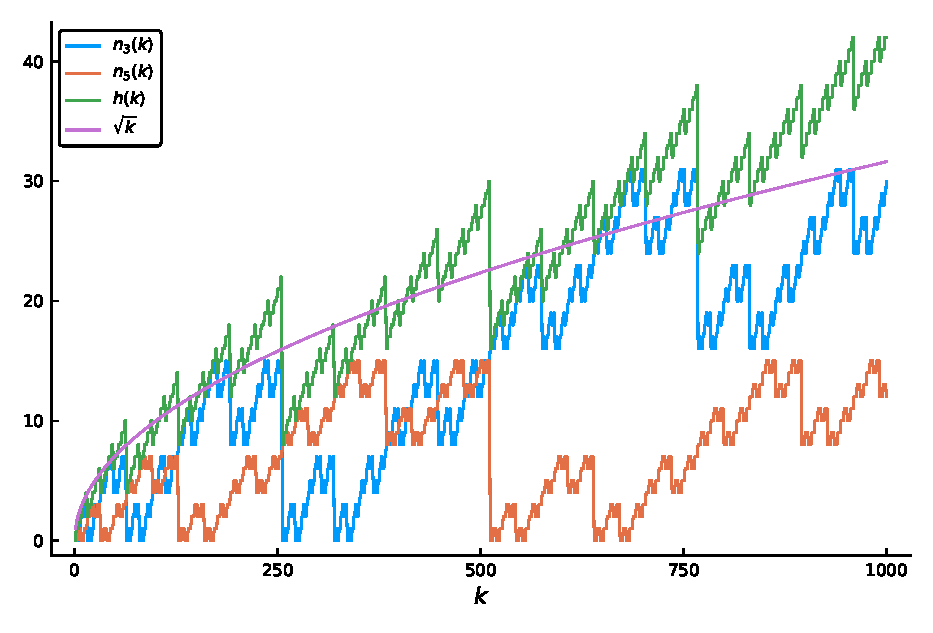
\includegraphics{behaviour_up_to_1000}
	
	(Plot with other scales in \ref{plot:Behaviour_h}.)
\end{center}

\subparagraph{Code's Behaviour}
It may be interesting to represent how the code grows according to both parameters.
First, we can make a small table of values:
\begin{center}
	\begin{tabular}{|c||c|c|c|c|c|c|c|c|c|c|c|}
		\hline
		\textbf{} & \textbf{0} & \textbf{1} & \textbf{2} & \textbf{3} & \textbf{4} & \textbf{5} & \textbf{6} & \textbf{7} & \textbf{8} & \textbf{9} & \textbf{10} \\\hline\hline
		\textbf{0} & 0 & 4 & 16 & 20 & 64 & 68 & 80 & 84 & 256 & 260 & 272 \\
		\textbf{1} & 2 & 6 & 18 & 22 & 66 & 70 & 82 & 86 & 258 & 262 & 274 \\
		\textbf{2} & 8 & 12 & 24 & 28 & 72 & 76 & 88 & 92 & 264 & 268 & 280 \\
		\textbf{3} & 10 & 14 & 26 & 30 & 74 & 78 & 90 & 94 & 266 & 270 & 282 \\
		\textbf{4} & 32 & 36 & 48 & 52 & 96 & 100 & 112 & 116 & 288 & 292 & 304 \\
		\textbf{5} & 34 & 38 & 50 & 54 & 98 & 102 & 114 & 118 & 290 & 294 & 306 \\
		\textbf{6} & 40 & 44 & 56 & 60 & 104 & 108 & 120 & 124 & 296 & 300 & 312 \\
		\textbf{7} & 42 & 46 & 58 & 62 & 106 & 110 & 122 & 126 & 298 & 302 & 314 \\
		\textbf{8} & 128 & 132 & 144 & 148 & 192 & 196 & 208 & 212 & 384 & 388 & 400 \\
		\textbf{9} & 130 & 134 & 146 & 150 & 194 & 198 & 210 & 214 & 386 & 390 & 402 \\
		\textbf{10} & 136 & 140 & 152 & 156 & 200 & 204 & 216 & 220 & 392 & 396 & 408 \\
		\hline
	\end{tabular}

	Table in of (even) integers corresponding to code $[line,column]$.
\end{center}
(Larger table in \ref{table:CodeToIntegers}.)

But it isn't very visual, so another way to view it is as a surface (obtained by linking with triangles the points plotted).
On the grid $\left[ 0,10 \right]^2$, we plot the surface $z = \left[ x, y \right]$ i.e. $z$ is the integer with code $\left[ x, y \right]$.
\begin{center}
	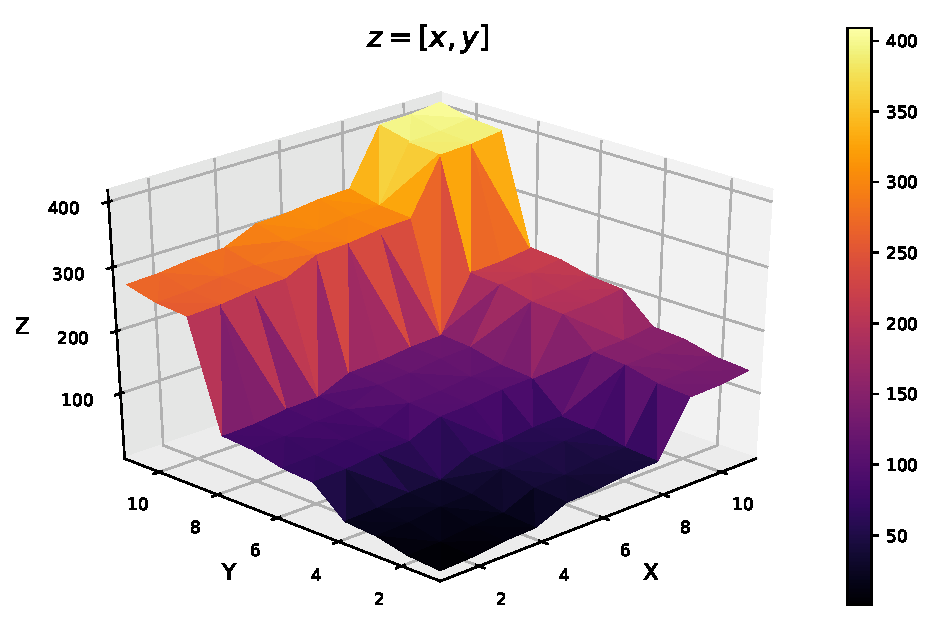
\includegraphics{code_plot_10-10}
	
	Plot of the surface with height given by the code of $X$ and $Y$.\\
	(i.e. the surface with equation $Z = [X,Y]$.)
\end{center}
(Other scales of plots available in \ref{plot:CodeSurface}.)

\paragraph{Order Relation}
We define the following order relation on natural numbers:
For $m, l \in \N$, $m \prec l$ if $h(m) < h(l)$ or $h(m) = h(l)$ and $n_5(m) \prec n_5(l)$.
This relation is a total order, this is straightforward to check.

\subsubsection{Action of $T_3$ and $T_5$}
\paragraph{$h$ on modular forms}
For the rest of the section, we will write a modular form $f \in \mathcal{F}$ as follows:
$f = \Delta^{m_1} + \Delta^{m_2} + \dots + \Delta^{m_r}$ with $m_1 > m_2 > \dots > m_r$.
In this case, $m_1$ is the \textit{degree} of $f$, and we will denote it by $\degree{f}$.
We write $\degree{f} = -\infty$ if $f=0$.
We define $h(f) = h(m_1)$, and $h(f) = -\infty$ if $f=0$.
Similarly, we define $n_3(f) = n_3(m_1)$ and $n_5(f) = n_5(m_1)$, and $n_3(f) = n_5(f) = -\infty$ if $f=0$.

\paragraph{Action of $T_3$}
Here, we want to give a description for the behaviour of $h(T_3|f)$ and $\degree{T_3|f}$.
\label{propositionActionT3}
\begin{proposition}
	Let $f \in \mathcal{F}$ be a non-zero modular form modulo 2.
	\begin{enumerate}
		\item In general, $h(T_3|f) \leq h(f)-1$.
		\item If $n_3(f)>0$, then $h(T_3|f) = h(f)-1$ and $\degree{T_3|f}$ has code $\left[ n_3(f)-1, n_5(f) \right] $.
	\end{enumerate}
\end{proposition}
This proposition is stated in \cite[§4]{OrdreNilpotenceOperateurHecke}, and a complete proof is given in \cite{ModularFormsMcGill}.

\paragraph{Action of $T_5$}
Similarly to the above for $T_3$, we want to give a description for the behaviour of $h(T_5|f)$ and $\degree{T_5|f}$.
\label{propositionActionT5}
\begin{proposition}
	Let $f \in \mathcal{F}$ be a non-zero modular form modulo 2.
	\begin{enumerate}
		\item In general, $h(T_5|f) \leq h(f)-1$.
		\item If $n_5(f)>0$, then $h(T_5|f) = h(f)-1$ and $\degree{T_5|f}$ has code $\left[ n_3(f), n_5(f)-1 \right] $.
	\end{enumerate}
\end{proposition}
Again, this proposition is stated in \cite[§4]{OrdreNilpotenceOperateurHecke}, and a complete proof is given in \cite{ModularFormsMcGill}.



\subsubsection{Formula for the Order of Nilpotency}
\paragraph{Lower bound}
\begin{property}
	Let $f \in \mathcal{F}$ be a non-zero modular form modulo 2 of degree $m_1$.
	Then we have:
	$$
	T_3^{n_3(m_1)} T_5^{n_5(m_1)} | f = \Delta
	$$
\end{property}
\begin{proof}
	We apply $n_3(m_1)$ times the proposition about $T_3$ above, and $n_5(m_1)$ times the proposition about $T_5$, to get that the degree of $g = T_3^{n_3(m_1)}T_5^{n_5(m_1)}|f$ has code $\left[ 0,0 \right]$.
	The propositions also implies that $h(g) > -\infty$, i.e. $g \neq 0$.
	Therefore, $\degree{g} > -\infty$, so it must be odd. since it has code $\left[ 0,0 \right]$,  $\degree{g} = 1$, thus $g = \Delta$.
\end{proof}

\begin{corollary}
	Let $f \in \mathcal{F}$ be a non-zero modular form modulo 2.
	We have $g(f) \geq h(f) +1$.
\end{corollary}
\begin{proof}
	This is directly implied by the proposition:
	As $T_3^{n_3(m_1)}T_5^{n_5(m_1)}|f = \Delta \neq 0$, we have $g(f) \geq n_3(f)+n_5(f)+1 = h(k)+1$.
\end{proof}

\paragraph{Representation of $\mathcal{F}$}
\subparagraph{Table}
This means that for each $k$ odd, there is pair $\left[ a,b \right] = \left[ n_3(k),n_5(k) \right] \in \N\times\N$ (which corresponds to the code of $k$), such that $T_3^aT_5^b|\Delta^k = \Delta$.
Explicitly, $T_3^{n_3(k)}T_5^{n_5(k)}|\Delta^k = \Delta$.
Thus, we can arrange all odd powers of the discriminant $\Delta$ in a table, such that applying the corresponding Hecke operators give exactly $\Delta^1$:
\begin{center}
	\begin{tabular}{|c||ccccccccccc|}
		\hline
		\textbf{} & \textbf{$T_5^{0}$} & \textbf{$T_5^{1}$} & \textbf{$T_5^{2}$} & \textbf{$T_5^{3}$} & \textbf{$T_5^{4}$} & \textbf{$T_5^{5}$} & \textbf{$T_5^{6}$} & \textbf{$T_5^{7}$} & \textbf{$T_5^{8}$} & \textbf{$T_5^{9}$} & \textbf{$T_5^{10}$} \\
		\hline\hline
		$T_3^{0}$ & $\Delta^{1}$ & $\Delta^{5}$ & $\Delta^{17}$ & $\Delta^{21}$ & $\Delta^{65}$ & $\Delta^{69}$ & $\Delta^{81}$ & $\Delta^{85}$ & $\Delta^{257}$ & $\Delta^{261}$ & $\Delta^{273}$ \\
		$T_3^{1}$ & $\Delta^{3}$ & $\Delta^{7}$ & $\Delta^{19}$ & $\Delta^{23}$ & $\Delta^{67}$ & $\Delta^{71}$ & $\Delta^{83}$ & $\Delta^{87}$ & $\Delta^{259}$ & $\Delta^{263}$ & $\Delta^{275}$ \\
		$T_3^{2}$ & $\Delta^{9}$ & $\Delta^{13}$ & $\Delta^{25}$ & $\Delta^{29}$ & $\Delta^{73}$ & $\Delta^{77}$ & $\Delta^{89}$ & $\Delta^{93}$ & $\Delta^{265}$ & $\Delta^{269}$ & $\Delta^{281}$ \\
		$T_3^{3}$ & $\Delta^{11}$ & $\Delta^{15}$ & $\Delta^{27}$ & $\Delta^{31}$ & $\Delta^{75}$ & $\Delta^{79}$ & $\Delta^{91}$ & $\Delta^{95}$ & $\Delta^{267}$ & $\Delta^{271}$ & $\Delta^{283}$ \\
		$T_3^{4}$ & $\Delta^{33}$ & $\Delta^{37}$ & $\Delta^{49}$ & $\Delta^{53}$ & $\Delta^{97}$ & $\Delta^{101}$ & $\Delta^{113}$ & $\Delta^{117}$ 
		& $\Delta^{289}$ & $\Delta^{293}$ & $\Delta^{305}$ \\
		$T_3^{5}$ & $\Delta^{35}$ & $\Delta^{39}$ & $\Delta^{51}$ & $\Delta^{55}$ & $\Delta^{99}$ & $\Delta^{103}$ & $\Delta^{115}$ & $\Delta^{119}$ 
		& $\Delta^{291}$ & $\Delta^{295}$ & $\Delta^{307}$ \\
		$T_3^{6}$ & $\Delta^{41}$ & $\Delta^{45}$ & $\Delta^{57}$ & $\Delta^{61}$ & $\Delta^{105}$ & $\Delta^{109}$ & $\Delta^{121}$ & $\Delta^{125}$ & $\Delta^{297}$ & $\Delta^{301}$ & $\Delta^{313}$ \\
		$T_3^{7}$ & $\Delta^{43}$ & $\Delta^{47}$ & $\Delta^{59}$ & $\Delta^{63}$ & $\Delta^{107}$ & $\Delta^{111}$ & $\Delta^{123}$ & $\Delta^{127}$ & $\Delta^{299}$ & $\Delta^{303}$ & $\Delta^{315}$ \\
		$T_3^{8}$ & $\Delta^{129}$ & $\Delta^{133}$ & $\Delta^{145}$ & $\Delta^{149}$ & $\Delta^{193}$ & $\Delta^{197}$ & $\Delta^{209}$ & $\Delta^{213}$ & $\Delta^{385}$ & $\Delta^{389}$ & $\Delta^{401}$ \\
		$T_3^{9}$ & $\Delta^{131}$ & $\Delta^{135}$ & $\Delta^{147}$ & $\Delta^{151}$ & $\Delta^{195}$ & $\Delta^{199}$ & $\Delta^{211}$ & $\Delta^{215}$ & $\Delta^{387}$ & $\Delta^{391}$ & $\Delta^{403}$ \\
		$T_3^{10}$ & $\Delta^{137}$ & $\Delta^{141}$ & $\Delta^{153}$ & $\Delta^{157}$ & $\Delta^{201}$ & $\Delta^{205}$ & $\Delta^{217}$ & $\Delta^{221}$ & $\Delta^{393}$ & $\Delta^{397}$ & $\Delta^{409}$ \\
		\hline
	\end{tabular}

	Table of powers $\Delta^k$ such that the corresponding operator applied to $\Delta^k$ gives $\Delta^1$.\\
	(i.e. $\Delta^k$ such that $T_3^{line}T_5^{column}|\Delta^k = \Delta$.)
\end{center}
(A larger table can be found in \ref{table:OperatorToDelta1}.)

From the fact that codes are in bijection with odd integers, we can use this table as a basis for modular forms modulo 2.


\paragraph{Exact Formula}
We derive here an explicit formula for the order of nilpotency of a modular form modulo 2.
\label{theoremOrderOfNilpotency}
\begin{theorem}[Order of Nilpotency of Modular Forms Modulo 2] \cite[§5]{OrdreNilpotenceOperateurHecke}.
	Let $f \in \mathcal{F}$ be a non-zero modular form modulo 2.
	The order of nilpotency is exactly $g(f) = h(f) + 1$.
\end{theorem}
What remains to prove is that $g(f) \leq h(f) + 1$.
This is proved in \cite[§5]{OrdreNilpotenceOperateurHecke}.

From this follows a new remark, which is useful to estimate computations times:
As $g(f)=h(f)+1$, and $h(f) = h(\degree{f}) = \mathcal{O}(\sqrt{\degree{f}})$, we have $g(f) = \mathcal{O}(\sqrt{\degree{f}})$, i.e. the nilpotency order of a modular form behaves asymptotically as the square root of its degree.

\label{corollaryOrderOfNilpotency}
\begin{corollary}
	Let $f \in \mathcal{F}$ be a non-zero modular form modulo 2.
	If $T_3|f = T_5|f = 0$, then $f = \Delta$.
\end{corollary}
\begin{proof}
	By the previous proposition, we have both $n_3(f)=0$ and $n_5(f)=0$.
	Thus, $\degree{f}$ has code $\left[ 0,0 \right]$.
	Since $f \neq 0$ and $f \in \mathcal{F}$, this means $f = \Delta$.
\end{proof}
